\documentclass[landscape, two column, full page,reqno]{article}
\usepackage{mathrsfs}
\usepackage{amsmath,amssymb,amsthm}
\usepackage[adobe-garamond]{mathdesign}
\AtBeginDocument{%
  \let\mathbb\relax
  \DeclareMathAlphabet\PazoBB{U}{fplmbb}{m}{n}%
  \newcommand{\mathbb}{\PazoBB}%
  \let\mathcal\relax
  \DeclareMathAlphabet{\OMScal}{OMS}{cmsy}{m}{n}
  \newcommand{\mathcal}{\OMScal}%
}
\usepackage{fitch}
\usepackage{enumitem}
\usepackage{fontspec}
\usepackage{tikz}
\usetikzlibrary{arrows}
\usepackage{multicol}
\setmainfont[Numbers={Proportional,OldStyle}]{Adobe Garamond Pro}
%NATBIB
\usepackage[comma]{natbib}
%HYPERREF PACKAGE
\usepackage{xcolor}
\PassOptionsToPackage{hyphens}{url}
\usepackage[backref=page,linktocpage=true,colorlinks]{hyperref}
\renewcommand{\backrefxxx}[3]{[\hyperlink{page.#1}{#1}]}
\hypersetup{
    colorlinks = true,
    citecolor = blue,
    urlcolor = blue,
    filecolor = blue,
    linkcolor = blue,
}
%PATCH TO ONLY HYPERLINK YEAR OF CITATION
\usepackage{etoolbox}
\makeatletter
% Patch case where name and year are separated by aysep
\patchcmd{\NAT@citex}
  {\@citea\NAT@hyper@{%
     \NAT@nmfmt{\NAT@nm}%
     \hyper@natlinkbreak{\NAT@aysep\NAT@spacechar}{\@citeb\@extra@b@citeb}%
     \NAT@date}}
  {\@citea\NAT@nmfmt{\NAT@nm}%
   \NAT@aysep\NAT@spacechar\NAT@hyper@{\NAT@date}}{}{}
% Patch case where name and year are separated by opening bracket
\patchcmd{\NAT@citex}
  {\@citea\NAT@hyper@{%
     \NAT@nmfmt{\NAT@nm}%
     \hyper@natlinkbreak{\NAT@spacechar\NAT@@open\if*#1*\else#1\NAT@spacechar\fi}%
       {\@citeb\@extra@b@citeb}%
     \NAT@date}}
  {\@citea\NAT@nmfmt{\NAT@nm}%
   \NAT@spacechar\NAT@@open\if*#1*\else#1\NAT@spacechar\fi\NAT@hyper@{\NAT@date}}
  {}{}
\makeatother
%
%Titlesec package
\usepackage{titlesec}
%Centering and readjusting size of headings
\titleformat{\section}[hang]
{\normalfont\sc\filcenter}{\thesection}{1em}{}
\titleformat{\subsection}[hang]
{\normalfont\sc\filcenter}{\thesubsection}{1em}{}
\titleformat{\subsubsection}[hang]
{\normalfont\sc\filcenter}{\thesubsubsection}{1em}{}
			% in the document preamble: 
				\let\endgraf\par % because LaTeX doesn't like \par 
			% in some command arguments 
				\let\subtitlefont\normalfont % or whatever 
				
%FOOTNOTE SPACING
\usepackage[hang,multiple,splitrule]{footmisc}
\setlength{\footnotemargin}{4mm}

\newcommand{\qd}{\begin{quote}\begin{description}  [align=left,style=nextline,leftmargin=*,labelsep=0pt,font=\normalfont]}
\newcommand{\zd}{\end{description}\end{quote}}
\newcommand{\qe}{\begin{enumerate}[align=left,style=nextline,leftmargin=17pt,labelsep=5pt,font=\normalfont]}
\newcommand{\qer}{\begin{enumerate}[align=left,style=nextline,leftmargin=17pt,labelsep=5pt,font=\normalfont , resume]}
\newcommand{\qei}{\begin{enumerate}[align=left,style=nextline,leftmargin=15pt, labelsep=10pt,font=\normalfont]}
\newcommand{\ze}{\end{enumerate}}
\newcommand{\p}{\item}
\newcommand{\e}{\emph}
\newcommand{\s}{\textsc}
\newcommand{\tbf}{\textbf}
\newcommand{\fn}{\footnote}
\newcommand{\argu}[2]{\begin{center}\begin{minipage}{#1} \begin{enumerate}
	#2
\end{enumerate}
\end{minipage}  
\end{center}}
\newcommand{\qq}[1]{ ~\!^\ulcorner #1  ^\urcorner~\!}
\newcommand{\V}[1]{\llbracket #1 \rrbracket}
\newcommand{\D}{\mathcal{D}}
\newcommand{\W}{\mathcal{W}}
\renewcommand{\u}{\mathfrak{u}}
\newcommand{\df}{\stackrel{\text{\tiny def}}{=}}
\newcommand{\fproof}[1]{\begin{center}\begin{fitch} #1 \end{fitch}\end{center}}
%GRAPHICX PACKAGE
\usepackage{graphicx}
\graphicspath{{/Users/jdg83/Desktop/Figures/}}
\usepackage{xcolor}
\usepackage{fancybox}

\definecolor{ShadowColor}{RGB}{30,150,190}

\makeatletter
\newcommand\Cshadowbox{\VerbBox\@Cshadowbox}
\def\@Cshadowbox#1{%
  \setbox\@fancybox\hbox{\fbox{#1}}%
  \leavevmode\vbox{%
    \offinterlineskip
    \dimen@=\shadowsize
    \advance\dimen@ .5\fboxrule
    \hbox{\copy\@fancybox\kern.5\fboxrule\lower\shadowsize\hbox{%
      \color{gray}\vrule \@height\ht\@fancybox \@depth\dp\@fancybox \@width\dimen@}}%
    \vskip\dimexpr-\dimen@+0.5\fboxrule\relax
    \moveright\shadowsize\vbox{%
      \color{gray}\hrule \@width\wd\@fancybox \@height\dimen@}}}
\makeatother

\newcommand{\csbox}[2]{\begin{center}
\Cshadowbox{
\begin{minipage}{#1}
	#2
\end{minipage}}
\end{center}
}


\title{Kripke, \e{Naming and Necessity}}
\date{September 11th, 2018}
\author{M\e{{\fontspec{Minion Pro} \&}}E Core}

\usepackage{layout}
\voffset = -40pt
\textheight = 450pt
\setlength{\columnsep}{20pt}
\begin{document}
%\layout
\twocolumn[{%
 \centering
\maketitle
}]

\section{Stage Setting}
\subsection{Speaking of Non-Actual Possibilities}
\qe

\p A riddle with an important lesson: if `tail' meant leg, how many tails would a horse have?
	\qe
	\p Correct answer: one.  If we had spoken a different language, this on its own would not have changed anything about the world---and, in particular, it would not have given horses any more tails.  Of course, if `tail' meant leg, the sentence `a horse has four tails' would be true.  But this is a very different claim that the claim that, if `tail' meant leg, a horse would have four tails.
	\p Compare: If `2' meant 4 and `4' meant 2, then `2+2=4' would not be true, though 2+2 would still be 4.  It is a necessary truth that 2+2=4, not a contingent matter we have the ability to change by simply changing the way we speak.  By changing the way we speak, we could change a true sentence into a false one; but we would not thereby make 2+2 $\neq$ 4.
	\p Lesson: when we discuss a non-actual possibility, we do not `go native' and adopt the language of the inhabitants of that non-actual possibility.  Rather, when we discuss a non-actual possibility, we continue speaking our actual language in describing that possibility.
	\ze 
	
\subsection{Metaphysical and Epistemic Possibility}

\p We should carefully distinguish between things which are \e{metaphysically} possible and things which are \e{epistemically} possible.  This can lead to confusion, since we are able to express both brands of possibility with the words `might' and `must'. 
	\qe
	\p   However, we can see that metaphysical and epistemic possibility come apart by noting the felicity of dialogues like the following:
		\begin{quote}
		Goldbach's conjecture might be true, and it might not be true---we don't yet know.  However, since it is a mathematical claim, it's not contingent.  It is either necessarily true or it is necessarily false.
		\end{quote}
	\p This is an eminently sensible thing to say, but, in order to make sense of it, we will have to distinguish two different brands of modality.  For if we interpret this speech as making the following two claims,
			\begin{align*}
			&\Diamond G \wedge \Diamond \neg G		\\
			&\Box G \vee \Box \neg G
			\end{align*}
	then we will have contradicted ourselves.\footnote{ Since `$\Diamond$' is short for `$\neg \Box \neg$', the first claim is equivalent to `$\neg \Box \neg G \wedge \neg \Box G$', which is equivalent to `$\neg( \Box \neg G \vee \Box G)$'.}
	\p The solution is to recognize two different meanings for `might'.  There is an \e{epistemic} use of `might', meaning roughly `for all we know'.\footnote{ This is far too rough.  There is now a massive literature on the semantics of the epistemic use of `might', but it's outside of the purview of this class.}  It is in this sense that Goldbach's conjecture might be true and might be false.  And there is a \e{metaphysical} use of `might', meaning that there is some genuine way for the proposition to be true.  It is in this sense that Goldbach's conjecture is either necessarily true or necessarily false.
	\ze 
	
\subsection{Rigid Designation}	

\p We will use the term `designator' neutrally for any kind of referring expression.  So both `the morning star' and `Hesperus' are \e{designators}.   The first kind of designator we will call a \e{definite description}.  The second kind of designator we will call a \e{name} (or, a \e{proper name}).

\p A designator is \e{rigid} iff the designator refers to the same thing in every possible world (in which the designator refers to anything at all)---or, perhaps more perspicaciously, iff there are no two possible worlds such that the designator refers to different things in each of those two possible worlds.  A designator is \e{non-rigid} iff it is not rigid---\e{i.e.}, iff there \e{are} two possible worlds such that the designator refers to two different things in each of those possible worlds.
	\qe
	\p For a relatively uncontroversial example of a non-rigid designator, consider ``the inventor of bifocals''.  In the actual world, this refers to Ben Franklin.  However, there are other possible worlds in which Franklin didn't invent bifocals at all, and they were instead invented by Thomas Jefferson.  In those possible worlds, ``the inventor of bifocals'' refers to Jefferson.
		\qe
		\p Note that we need to be careful that we are not making the mistake of `going native'.  While it's true that the inhabitants of that world would use ``the inventor of bifocals'' to refer to Jefferson, that's not the question we ask ourselves when deciding whether the designator is non-rigid.  We ask ourselves whether, when \e{we} describe that counterfactual state-of-affairs, in \e{our} language, we say that it is a possibility in which Jefferson is the inventor of bifocals.
		\ze 
	\p For a relatively uncontroversial example of a rigid designator, consider the numeral ``2''.  This numeral refers to the same thing---namely, the number 2---in every possible world.  
		\qe
		\p Again, of course there are possible worlds in which people use the symbol ``2'' to refer to things other than the number 2.  But we don't `go native'.  We ask whether, when \e{we} talk about that possible world, \e{we} are talking about the number 2. 
		\ze 
	\ze 
\p There is a wrinkle here concerning possible worlds in which the referent of a designator does not exist which Kripke mostly irons over (and we, for the most part, will iron over as well).  But let us at least mention it before sweeping it under the rug.
	\qe
	\p Consider the rigid designator ``Rigid Trump''.  I introduce the designator  ``Rigid Trump'' as follows: the name refers to Trump, and does so rigidly.\footnote{ If Kripke is right, then ``Rigid Trump'' is synonymous with ``Trump''.  But we don't need to settle this question in order to discuss these issues.}  Now, consider a possible world where Trump does not exist.  Does ``Rigid Trump'' still refer to Trump?  
	\p On the one hand, it seems that it should not, since, at this possibility, Rigid Trump doesn't exist.  So there's nothing \e{at} that possibility for ``Rigid Trump'' to refer to.
	\p However, on the other hand, I just said that Rigid Trump doesn't exist.  So it looks like I need to be able to say that 
					\[
					\neg (\exists x) (x = \text{ Rigid Trump})
					\]
		But, in order for this sentence to have a truth-value at that world, we need ``Rigid Trump'' to refer to something, and, moreover, to refer to something which doesn't exist at that world.
	\p There are lots of subtle issues here, and to fully address them, we would have to talk about quantified modal logic, free logic, empty names in general, and get into lots of other messy debates.  Fortunately, our definition of `rigid designator' need not, and does not, take a stand on this question.
	\ze 
\p One of Kripke's primary goals is to argue that proper names are rigid designators.  Since he takes it to be uncontroversial and common ground that definite descriptions are \e{not} rigid designators, this allows him to conclude that proper names are not synonymous with any definite description, or any disjunction of definite descriptions.  


\subsection{Descriptivism}

\p Suppose that we introduce the meaning of `1 meter' by pointing to a certain stick and saying `A meter will be the length of this stick (now)'.   We have here used a definite description `the length of this stick (now)', to introduce the meaning of `1 meter'.  But this could have been done in one of two ways.  
	\qe
	\p We could have used the definite description to \e{fix the reference} of `1 meter'; or,
	\p We could have used it to \e{give the meaning} of `1 meter'.
	\ze  
or, of course, we could have done \e{both}.  
\p \e{Descriptivism} is the view that definite descriptions like `the morning star' and `the evening star' are both used the fix the reference of proper names like `Hesperus' and `Phosphorus', \e{and} to give the meaning of proper names like `Hesperus' and `Phosphorus'.
	\qd
	\p[\s{Metasemantic Descriptivism}] The reason why a proper name refers to its referent is that the referent satisfies some definite description. For instance, the reason `Hesperus' refers to Venus is that Venus is the first star visible in the evening (hereafter: `the evening star').
	\p[\s{(Semantic) Descriptivism}] Proper names are synonymous with definite descriptions.  For instance, `Hesperus' is synonymous with `the evening star'.
	\zd 
	\qe
	\p  If we interpret Fregean senses as definite descriptions, then Frege was committed to both forms of Descriptivism.
	\p If we are using the possible worlds framework to try to solve Frege's puzzle (as we saw last week), then we are supposing that the meaning of `Hesperus $=$ Phosphorus' is a contingent function from possible worlds to truth-value which is synonymous with `the morning star $=$ the evening star'.  So we are at least committed to \e{Semantic} Descriptivism.
	\ze 
	
\subsection{The Necessity of Identity}

\p Kripke accepts a principle of quantified modal logic with identity called the \e{necessity of identity}.  This is the thesis that the following is a logical truth:
			\[\tag{$\Box =$}\label{ni}
			(\forall x) (\forall y) (x = y \to \Box x = y)
			\]
			\qe
			\p Kripke notes that the necessity of identity follows from the premise that everything is necessarily \e{self}-identical and Leibniz's Law.  Here's a Fitch-style proof:
			\ze 
			
			\vspace{-20pt}
			
			\fproof{
			\fa (\forall x) \Box x=x				&						\\
			\fj (\forall F)(\forall x)(\forall y) (x=y \to (Fx \to Fy))			&			\\
			\fa	(\forall x)(\forall y)(x=y \to (\Box x=x \to \Box x=y)))		&	2, $\forall E [F$\underline{~~~} $\to \Box x=$\underline{~~~}$]$	\\
			\fa (\forall y)(h=y \to (\Box h=h \to \Box a=y))												&3, $\forall E[x \to h]$		\\
			\fa h=p \to (\Box h=h \to \Box h=p)												&	4, $\forall E[y \to p]$	\\
			\fa \fh h=p																							& Assumption	\\
			\fa \fa \Box h=h \to \Box h=p															& 5, 6, $MP$	\\
			\fa \fa \Box h=h																					& 1, $\forall E[x \to h]$\\
			\fa \fa \Box h=p																					& 7, 8, $MP$	\\
			\fa h=p \to \Box h=p																			& 6--9, $\to I$	\\
			\fa (\forall y)(h = y \to \Box h=y)													& 10, $\forall I[p \to y]$	\\
			\fa (\forall x)(\forall y)(x=y \to \Box x=y)									& 11, $\forall I[h \to x]$
			}
\p Suppose that we use `$h$' as a logical constant for Hesperus, and we use `$p$' as a logical constant for Phosphorus.  If we accept the necessity of identity, and we accept the usual rules for the quantifiers, then we should accept 	`$h=p \to \Box h=p$'.  Moreover, we should accept `$h=p$'.  So, if we accept \e{modus ponens}, then we should accept  `$\Box h=p$'.
	\qe
	\p What does this show?  It shows that, if we accept that $(\forall x) \Box x=x$ and we accept Leibniz's law in our logical language, then, \e{in our logical language}, singular terms are rigid designators.  If the singular terms `$h$' and `$p$' actually refer to the same thing, so that `$h=p$' is true, then they must \e{necessarily} refer to the same thing, so that `$\Box h=p$' is true.
	\p It does \e{not} show that \e{in English}, proper names are rigid designators.  In particular, it does not show that `$h$' in our logical language is synonymous with `Hesperus' in English.  It could be that much is lost in translation into logic.
	\ze
\p To see this more clearly, let's think about outfitting our logical language with definite descriptions, so that it includes the designators `the morning star' and `the evening star'.  Then,  the following \e{substitution instance} of \eqref{ni} would be false:
				\[
				\text{ the morning star } = \text{ the evening star } \to \Box \text{ the morning star } = \text{ the evening star }
				\]
			\qe
			\p The truth of \eqref{ni} in our \e{logical} language doesn't tell us that `the morning star' and `the evening star' are rigid designators \e{in English}.  And similarly, it doesn't tell us that `Hesperus' and `Phosphorus' are rigid designators \e{in English}.
			\ze 
\p A brief digression: the present case illustrates an important distinction between two different ways of understand the quantifiers $\forall$ and $\exists$.
	\qe
	\p On a \e{substitutional} understanding of the quantifiers, `$\exists x Fx$' is true iff there is some \e{designator}, $d$, such that, when we substitute `$d$' for `$x$' in `$Fx$'---arriving at `$Fd$', we get a truth.
\p On an \e{objectual} understanding of the quantifiers, `$\exists x Fx$' is true iff there is some entity such that, if we allow `$x$' to \e{directly refer} to that entity, then `$Fx$' is true.
	\qe
	\p This is accomplished with the aid of a \e{variable assignment} function, $g$.  Our semantics say that `$\exists x Fx$' is true in the model $\mathcal{M}$, with variable assignment $g$, iff there is some thing $u$ in the domain such that `$Fx$' is true in the model $\mathcal{M}$, with the \e{variant} variable assignment $g_{x \to u}$, where $g_{x \to u}$ is exactly like $g$, except that `$x$' now refers to $u$ (if it didn't already). 
	\ze 
	\p Note that, once we've outfitted our logical language with definite descriptions, on a substitutional understanding of the quantifiers, \eqref{ni} would be false, since it has a false substitution instance.  However, on an objectual understanding of the quantifiers, \eqref{ni} would still be true. 
	\ze 



\section{Kripke's Arguments Against Descriptivism}
\p Kripke gives three different arguments against Descriptivism: a \e{modal} argument, a \e{semantic} argument, and an \e{epistemic argument}.
\section{The Modal Argument}
\p By the compositionality of meaning, substitution of synonymous expressions within a sentence should not affect the meaning---and certainly not the truth-value---of the entire sentence.  

 Yet the following two claims differ in truth-value.  The first is true, the second false.
		\qe
		\p Necessarily, Hesperus $=$ Phosphorus.\label{a}
		\p Necessarily, the evening star $=$ the morning star.\label{b}
		\ze 
 Similarly, the first claim below is true, the second false.
		\qer
		\p Possibly, Hesperus $\neq$ the evening star.\label{c}
		\p Possibly, the evening star $\neq$ the evening star.\label{d}
		\ze 
 Similarly, the first claim is true, the second false.
		\qer
		\p If Venus were smaller,\footnote{ I am supposing that, if Venus were smaller, then it wouldn't be as bright, and other stars would be visible before it was.} then Hesperus would not be the evening star.
		\p If Venus were smaller, then the evening star would not be the evening star.
		\ze 
So, `Hesperus' is not synonymous with `the evening star'.
\p More generally, almost all definite descriptions\footnote{ \e{Almost} all, but not all.  Consider definite descriptions like `the only even prime'.  This will pick out the number 2 in every possible world.  And consider `the actual evening star'.  This will pick out the planet Venus in every possible world.} will be non-rigid.  But proper names are rigid, as we can see by noticing that the following claims are plainly true:
	\qe
	\p Einstein could have failed to discover the theory of relativity.
	\p Aristotle could have failed to go into Philosophy, could have failed to teach Plato or Alexander the Great, and could have been born somewhere other than Stagira.
	\ze 
But this means that `Einstein' cannot just mean `the man who discovered the theory of relativity'.  And `Aristotle' cannot just mean `the Philosopher who was born in Stagira and who taught Plato and Alexander the Great'.
\p We could try to salvage Semantic Descriptivism by changing the descriptions we claim are synonymous with proper names.  For instance, we might claim that, while `Hesperus' isn't synonymous with `the evening star', it \e{is} synonymous with `the \e{actual} evening star'.
	\qe
	\p Recall the lesson of the riddle `if `tail' meant leg, how many tails would a horse have?'.  When we consider non-actual states of affairs, we continue using our own language.  So, in particular, `actual' continues to refer to \e{our} world.  So, if we consider a world in which Venus is smaller, and we ask whether, in that world, the \e{actual} evening star is Hesperus, our answer should be `yes'.  The thing which is \e{actually} the evening star is Venus.  And Venus is necessarily Hesperus.  So, in the counterfactual state of affairs in which Venus is smaller, the actual morning star is Hesperus.
	\p The effect of including `actual' in our definite descriptions has been to \e{rigidify} those descriptions.  They now pick out the very same thing in every possible world.
	\p Let's call the view on which names are synonymous with \e{rigidified} definite descriptions \e{Rigidified (Semantic) Descriptivism}:
		\qd
		\p[\s{Rigidified (Semantic) Descriptivism}]  Proper names are synonymous with \e{rigidified} definite descriptions.  For instance, `Hesperus' is synonymous with `the \underline{actual} evening star'. 
		\zd 
	\ze 
\p Kripke's modal argument leaves both \s{Metasemantic Descriptivism} and \s{Rigidified Semantic Descriptivism} unscathed.  

\subsection{The Semantic Argument}

\p Kripke additionally gives an argument which targets \s{Metasemantic Descriptivism} and \s{Rigidified (Semantic) Descriptivism}.  Those arguments rely upon the following stories (the first and most famous of which is fictional, the second and third of which are actual):
	\qe
	\p A man named Schmidt first proved the incompleteness of arithmetic, though G\"odel found and published the manuscript.  As a result, everybody falsely believes that G\"odel proved the incompleteness of arithmetic.
	\p Though most credit Peano with first axiomatizing arithmetic, it was in fact Dedekind who first axiomatized arithmetic.
	\p Though Jonah existed, he was not swallowed by a whale, and, in fact, none of the things the Bible claims happened to Jonah in fact did.
	\ze 
\p These cases afford the following arguments against both \s{Metasemantic Descriptivism} and \s{Rigidified (Semantic) Descriptivism}:
	\qe
	\p  If there is any description most speakers associate with the name `G\"odel', it is `the (actual) man who first proved the incompleteness of arithmetic'.  If our fiction were actual, a (rigidified) descriptivist theory would claim that `G\"odel first proved the incompleteness of arithmetic' is true.  But, if our fiction were actual, then this claim would be false.  So a (rigidified) descriptivist theory is not correct.
		\qe
		\p Similarly, if metasemantic descriptivism were correct, then, in this fictional scenario the name `G\"odel' would be determined to refer to Schmidt.  But, in this fictional scenario, `G\"odel' would still refer to G\"odel.  So metasemantic descriptivism is false.
		\ze 
	\p If there is any description most speakers associate with the name `Peano', it is `the (actual) man who first axiomatized arithmetic'.  So, a (rigidified) descriptivism would claim that `Peano first axiomatized arithmetic' is true.  But this claim isn't true.  It was Dedekind, not Peano.  So a (rigidified) descriptivism is false.
		\qer
		\p Similarly, if metasemantic descriptivism were correct, then `Peano' would refer to Dedekind.  But `Peano' doesn't refer to Dedekind.  So metasemantic descriptivism is false.
		\ze 
	\p If there is any description most speakers associate with Jonah, it is that he was (actually) eaten by a whale.  So, if a (rigidified) descriptivism were correct, then `If Jonah existed, then he was eaten by a whale' would be true.  But this is not true.
		\qer
		\p Similarly, if metasemantic descriptivism were correct, then `Jonah' would have to refer to somebody who was eaten by a whale.  But it does not.  So metasemantic descriptivism is false.
		\ze 
	\ze 
	
\p In response to this argument, we might try to change the kinds of descriptions which we claim determine the reference and meaning of proper names.  For instance, we might try to say that `Aristotle' refers to the person who is called `Aristotle'.  Call this a \e{metalinguistic descriptivism}.
	\qd
	\p[\s{Metasemantic Metalinguistic Descriptivism}] The referent of a proper name, $\qq{N}$, is determined to be the thing which is called $\qq{N}$.  (That is: the reason why $\qq{N}$ refers to its referent is that its referent is called $\qq{N}$.)
	\p[\s{Semantic Metalinguistic Descriptivism}] A proper name, $\qq{N}$, is synonymous with the definite description $^\ulcorner$the person (actually) called `$N$'$^\urcorner$.
	\zd
	\qe
	\p Against this, Kripke argues that the metasemantic component of the theory will end up being circular.  For it says that the referent of $N$ is determined to be whatever thing is called `$N$'.  But in order to know what is called `$N$', I must first know to what the name `$N$' refers.
	\p Does Kripke give an argue against the semantic version of this view?  There can't be circularity worries about merely claiming that $\qq{N}$ and $\qq{\text{the person actually called `}N\text{'}}$ are synonymous, since such a claim doesn't offer any explanations which could be circular.  At the end of Lecture I (pp.~68--70), he points out that you could give similar semantic theses about any old word: `sages' just means `the people called `sages'', `quark' just means `the things called `quarks''.  Since these meaning claims are unsatisfying, we should similarly be unsatisfied with saying that $\qq{N}$ just means $\qq{\text{the person actually called `}N\text{'}}$.
	\ze 
\subsection{The Epistemic Argument}

\p As a final argument against descriptivism, Kripke objects that the view makes \e{a priori} a great many claims which are properly regarded as \e{a posteriori}.
	\qe
	\p If the meaning of `Aristotle' is `the (actual) teacher of Alexander the Great', then it should be \e{a priori} that Aristotle taught Alexander the Great.  But this is not \e{a priori}.  So the meaning of `Aristotle' is not `the (actual) teacher of Alexander the Great'.
	\ze 
\p Suppose that we think that the meaning of `Aristotle' is `the (actual) person called `Aristotle''.  Kripke suggests that even this will not be \e{a priori}, if we mean that somebody other than ourselves, in this instant, calls Aristotle `Aristotle'.

\subsection{Millianism and Causal-Historical Metasemantics}

\p One obvious alternative to descriptivism is the view that there is no more to the meaning of a proper name than its referent.  Let's call this view ``Millianism'', after J.S.~Mill, who apparently held the view.
	\qd
	\p[\s{Millianism}] The meaning of its proper name is its referent.
	\zd 
	\qe
	\p That is: the meaning of `Hesperus' is the same as the meaning of `Phosphorus'.  Thus, `Hesperus' and `Phosphorus' are synonymous.
	\ze 
\p Millianism is a \e{semantic} thesis---it is a thesis about the \e{meaning} of proper names.  There is another question, the \e{metasemantic} question, of how it comes to be that names acquire the meanings that they do.
	\qe
	\p With respect to this question, Kripke doesn't offer us a theory, but rather a \e{picture}.  The picture he offers goes like this: there is an initial baptism, at which somebody uses a name to refer to an individual.  From the initial baptism, the name is passed from speaker to speaker. So long as the causal links in this chain are appropriate, the name as used by speakers far down the causal chain will still refer to the person or thing named in that initial baptism.
	\p Some initial problems for this picture:  
		\qe
		\p Consider infants switched at birth.  Baby 1 is named `Samantha'.   Baby 2 is named `Sabeen'.  Then, Baby 1 is taken home by the wrong parents and called `Sabeen' for her whole life.  Similarly, Baby 2 is taken home by the wrong parents and called `Samantha' \e{her} whole life.  Kripke's theory tells us that, when Baby 1's friends say `Sabeen aced her math test', they are speaking about \e{Baby 2}.
		\p Consider the case of `gold' and `fool's gold'.  It could be that the first person to use the term `gold' was in fact talking about pyrite.  Kripke's theory predicts that  the stuff we think is gold (with atomic number 79) might not actually \e{be} gold, and the stuff we think is fool's gold (pyrite) might actually  be gold.\footnote{ Note: these `might's are epistemic, not metaphysical.}
		\ze 
	\ze 
	
\section{The Necessary A Posteriori \& the Contingent A Priori}
\p So Kripke has given powerful arguments that we should think that `Hesperus' and `Phosphorus' refer to the same thing in every possible world---that is, that they have the same \e{intension}.
	\qe
	\p But giving `Hesperus' and `Phosphorus' different intensions was our way of explaining the differences in cognitive significance between (\tbf{A}) and (\tbf{B}):
		\qe
		\p[(\tbf{A})] Hesperus $=$ Hesperus.
		\p[(\tbf{B})] Hesperus $=$ Phosphorus.
		\ze 
	If `Hesperus' and `Phosphorus' have the same intension, then (\tbf{A}) and (\tbf{B}) will have the same intension, too.   Bracketing worries about worlds where Venus doesn't exist, they will both be \e{necessarily} true.  So how can we account for the fact that (\tbf{A}) is \e{a priori} while (\tbf{B}) is \e{a posteriori}?
	\ze 
\p Kripke thinks that, even though (\tbf{B}) is \e{necessary}, it could still be \e{a posteriori}.
	\qe
	\p For another case of the necessary a posteriori, consider `water is $H_2O$'.  
	\p Firstly, let us establish that it is necessary that water is $H_2O$.  Now, of course, there are \e{epistemic} possibilities in which water is something other than $H_2O$, just as there are epistemic possibilities in which Goldbach's conjecture is false.  But these epistemic possibilities are not relevant to the question of whether it is \e{metaphysically} necessary that water is $H_2O$.  And also, of course there are possibilities in which a clear liquid other than $H_2O$ flows in the lakes and rivers, falls from the sky, sates thirst, and so on and so forth---call this clear liquid `$XYZ$'.   While these possibilities of course exist, it is wrong to describe them as possibilities in which \e{water} is $XYZ$.   And, of course, in these possibilities, the inhabitants may call $XYZ$ `water'---but remember the lesson of our riddle: we must take care to continue speaking our own language, and not fall into the customs and habits of the inhabitants of these worlds.    `Water' is a natural kind term---for Kripke, this means that it, like proper names, refers \e{rigidly}.  So it is necessary that water be $H_2O$.  
	\p Even though this is necessary, the only way to come to know that water is $H_2O$ is through empirical investigation.  Until you do some chemistry, you'll never know that water is $H_2O$.  So `water is $H_2O$ is \e{a posteriori}.
	\p So `water is $H_2O$', like `Hesperus $=$ Phosphorus', is necessary but \e{a posteriori}.
	\p Other examples fitting this same mold:
		\qe
		\p Gold has atomic number 79.
		\p There are no unicorns.
		\ze 
	\ze 

\p Similarly, Kripke thinks that there are propositions which are \e{contingent}, yet \e{a priori}.
	\qe
	\p For a case of the contingent a priori, consider the name `Julius'.  I introduce the name `Julius' as follows: \e{let `Julius' denote the inventor of the zipper (whoever they may be).}  Now that I have introduced the name `Julius' in this way, I am in a position to know the following:
		\qe
		\p[(\tbf{J})] If anybody invented the zipper, then Julius invented the zipper.
				\begin{figure}[t]
				\centering
				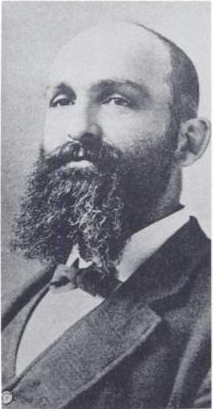
\includegraphics[width=40pt]{Julius.png}
				\caption{ Julius (a.k.a.~Whitcomb Judson)}
				\end{figure}
		\ze 
	\p	I know (\tbf{J}) to be true, just by knowing how the name  `Julius' was introduced by me.  I don't have to do any empirical investigation in order to discover that Julius invented the zipper if anybody did.  So (\tbf{J}) is \e{a priori}.
	\p Nevertheless, even though Julius \e{actually} invented the zipper, somebody else easily could have.  So there is a possible world in which somebody other than Julius invents the zipper, and (\tbf{J}) is false.  So (\tbf{J}) is contingent.
	\p So (\tbf{J}) is contingent and a priori.
	\p Other examples fitting this same mold: 
		\qe
		\p I am here now.
		\p Jack the Ripper committed the Whitechapel murders if anybody did.
		\p If there is a meter stick which determines the length of a meter, then the meter stick is one meter long.
		\ze 
	\ze
\ze 

\end{document}